\chapter{绪论}
\section{研究背景及意义}
\section{国内外研究现状}

在文献\cite{VATS}中,Li等人探讨了使用低成本超宽带设备 dwm1000 进行无设备的行人追踪问题。
作者提出了一种基于方差的时空映射算法(VATS),该算法把方差值映射到二维空间中的椭圆上,做为行人处于该椭圆的概率
并且从最大后验概率的角度解释了缓解干扰的原理。
此外,设计了一种粒子滤波算法来追踪位置可能性的变化。
实验结果表明,所提出的VATS映射算法实现了50th和90th百分位误差分别为0.156m和0.272m,
这对于实际应用来说是有希望的。


\section{本文主要工作}
\section{本文结构安排}

第一周       脚踢, 推进定位相关工作
第二周       国内外研究现状 ,研究背景及意义, 推进定位相关工作
第三周       相关技术(UWB,CNN LSTM), 完成定位除结论外的书写
第四周       相关技术(particle filter,聚类) 呼吸
\chapter{相关技术}
\section{UWB信道脉冲响应相关技术}
\section{深度学习相关技术}

\chapter{数据采集与预处理}
\section{引言}
\section{使用preamble归一化}
\section{上采样}
Decawave(Qorvo)的 DWM1000 和 NXP 的 NCJ29D5 设备的采样频率为 \(998.4 \, \text{MHz}\),对应的采样间隔为 \( \Delta \tau = 1.0016 \, \text{ns}\)。
电磁波在空气中的传播速度为 \(c = 299792458 \, \text{m/s}\),对应的波长为 \(\lambda = 0.2998 \, \text{m}\)。这个精度已经足够满足室内定位的需求。

然而,由于发送和接收设备之间的晶振并不能完全同步,导致接收到的信号的采样的相对开始时间不同步。
有一些研究者提出利用这一不同步来提高信号的采样频率,从而提高定位的精度~\cite{Ledergerber}。
也有一些研究者提出根据 IEEE 802.15.4a 规范~\cite{IEEE_Std_802.15.4a}, UWB CIR 的频谱几乎是矩形,因此可以利用 sinc 插值来提高信号的采样频率~\cite{MAMPI}。

本文借鉴了以上两种方法的思路,通过在频域中添加零来实现对信号的上采样,然后利用逆傅里叶变换(IFFT)将其转回到时域中,对结果取均值来叠加多帧的信息。下面将详细介绍上诉三种方法。

\subsection{均值滤波}
由于接收到的信号的采样的相对开始时间不同步,所以如果把λ分成多个等长的区间,每次采样只会落到其中的同一个区间,通过多次累加可以在每个区间内得到一个均值,从而提高采样率。

均值滤波算法通过以下形式的分段线性函数的系数 \( h = h_0 , h_1 , \ldots , h_{N_{\text{knots}} -1} \) 来跟踪当前测量的信道冲激响应(CIR)的均值:
\[ h(\tau ) = \frac{\tau  - \tau_i}{\Delta \tau_{\text{knots}}} h_i + \frac{\tau  - \tau_i}{\Delta \tau_{\text{knots}}} h_{i +1} \]
其中 \( i \) 满足 \( \tau_i \leq \tau < \tau_{i+1} \),并且 \( \Delta \tau_{\text{knots}} \) 是分段线性参数化的节点间的间隔。

分段线性参数化的节点 \( \tau_i \) 由以下公式给出:
\[ \tau_i = \tau_{\text{start}} + \Delta \tau_{\text{knots}} \cdot i \]
对于 \( i = \{0, \ldots , N_{\text{knots}} - 1\} \)。

节点总数 \( N_{\text{knots}} \) 由以下公式给出:
\[ N_{\text{knots}} = \frac{\tau_{\text{end}} - \tau_{\text{start}}}{\Delta \tau_{\text{knots}}} + 1 \]

分段线性函数表示CIR的均值计算复杂度低,该算法可以在每个DWM1000模块的主微控制器上运行,这对于实时处理至关重要,并且可以减少用于传输数据的空中时间。
由于其轻量化的特性,使其适用于具有有限内存和计算能力的嵌入式设备,并且可以实时执行。

\subsection{插值法}
本文主要使用了UWB的信道3与信道4。据IEEE 802.15.4a,UWB信道3的中心频率为4492.8Mhz,带宽为449.2Mhz,UWB信道4的中心频率为3993.6,带宽为1331.2Mhz。
信道3,4的频谱图像如图\ref{fig:spectrum_mask}所示,他们的频谱接近矩形,因此可以利用sinc插值来提高信号的采样频率。
\begin{figure}[htbp]
    \centering
    \includegraphics[width=.7\linewidth]{plotted/spectrum_mask}
    \caption{\label{fig:spectrum_mask}UWB信道3,4频谱}
\end{figure}

\begin{figure}[htbp]
    \centering
    \begin{subfigure}{0.33\textwidth}
        \centering
        \includegraphics[width=1.0\textwidth]{plotted/interpolation/time.png}
        \caption{\label{fig:time}原始时域图}
    \end{subfigure}%
    \begin{subfigure}{0.33\textwidth}
        \centering
        \includegraphics[width=1.0\textwidth]{plotted/interpolation/zero_time.png}
        \caption{\label{fig:zero_time}零填充后的时域图}
    \end{subfigure}
    \begin{subfigure}{0.33\textwidth}
        \centering
        \includegraphics[width=1.0\textwidth]{plotted/interpolation/sinc_time.png}
        \caption{\label{fig:sinc_time}sinc插值后的时域图}
    \end{subfigure}

    \begin{subfigure}{0.33\textwidth}
        \centering
        \includegraphics[width=1.0\textwidth]{plotted/interpolation/freq.png}
        \caption{\label{fig:freq}原始频域图}
    \end{subfigure}%
    \begin{subfigure}{0.33\textwidth}
        \centering
        \includegraphics[width=1.0\textwidth]{plotted/interpolation/zero_freq.png}
        \caption{\label{fig:zero_freq}零填充后的频域图}
    \end{subfigure}
    \begin{subfigure}{0.33\textwidth}
        \centering
        \includegraphics[width=1.0\textwidth]{plotted/interpolation/sinc_freq.png}
        \caption{\label{fig:sinc_freq}sinc插值后的频域图}
    \end{subfigure}
    \caption{sinc插值时频域图}
    \label{fig:interpolation}
\end{figure}

本文以信道3为例,介绍sinc插值的过程。

零填充:
首先,通过在原始数据样本(图\ref{fig:time})之间插入零,
对数据进行上采样。在每个原始数据样点之间插入 \( ( \text{upsample\_factor} - 1) \) 个零。
例如,如果上采样因子为4,那么在每个数据样点之间插入3个零,得到零填充后的时域图(图\ref{fig:zero_time})。
零填充的表达式如下所示:
\[
    x[n] = \{x[0], 0, 0, 0, x[1], 0, 0, 0, x[2], 0, 0, 0, \ldots\}
\]

从频域看,原始的频域图像(图\ref{fig:freq})变为零填充后的频域图像(图\ref{fig:zero_freq})。
为了使频域保持一致,需要通过在时域卷积sinc函数实现在频域的低通滤波。

构建 sinc 函数:
构建 sinc 函数以用于插值。sinc 函数是由以下公式定义的:
\[
    \text{sinc}(x) = \dfrac{\sin(\pi x)}{\pi x}
\]

在代码中,sinc 函数的参数是通过时域索引和上采样因子来调整的,以确保 sinc 函数正确对齐在零填充数据的样点上。

\[
    t = \text{np.arange}(-\text{len(zero\_padded\_data)}//2, \text{len(zero\_padded\_data)}//2) * 10^{-9}
\]
\[
    \text{sinc\_func} = \text{np.sinc}(\frac{t \cdot \text{cutoff\_frequency}}{\text{upsample\_factor} })
\]
其中zero\_padded\_data为零填充后的数据,upsample\_factor为上采样因子。
sinc函数的时频域图如\ref{fig:sinc}所示。
\begin{figure}[htbp]
    \centering
    \includegraphics[width=.7\linewidth]{plotted/interpolation/sinc.png}
    \caption{\label{fig:sinc}sinc函数时频图}
\end{figure}

卷积 (Convolution):
使用 sinc 函数对零填充的数据进行卷积,以得到插值的数据。这一步通过数学卷积操作完成,可以通过以下公式表示:
\[
    y[n] = \sum_{k=-\infty}^{\infty} x[k] \cdot \text{sinc\_func}[n - k]
\]

在代码中,这是通过 \texttt{np.convolve} 函数完成的:
\[
    \text{interpolated\_data} = \text{np.convolve}(\text{zero\_padded\_data}, \text{sinc\_func}, \text{mode}='same')
\]
从频域看,这相当于sinc函数与零填充数据的傅里叶变换的乘积,把零填充后的频域图(\ref{fig:zero_freq})转化为 sinc 插值后的频域图(\ref{fig:sinc_freq})。
从而在保证频域一致性的同时提高了时域的采样率

\subsection{fft法}
本文使用的fft法借鉴的sinc插值的原理,sinc插值是在时域上扩充信号,进行拟合,从而达到提高采样率的目的。
fft法直接在频域上进行修改,通过ifft变化得到时域的信号,从而达到提高时域采样率的目的。

\textbf{fft变换:}
首先通过fft把信号从图\ref{fig:time}变换到频域,得到图\ref{fig:freq}。
\[ X[k] = \text{FFT}\{ x[n] \} \]

\textbf{频域补零:}
然后在频域上插入零,得到图\ref{fig:sinc_freq}。这个操作相当于在时域进行上采样和sinc插值。对于4倍上采样,在频域中的每个非零点之间插入3个零,新的频域序列为:
\[ \tilde{X}[k] = \begin{cases}
X[k/4], & \text{if } k \mod 4 = 0 \\
0, & \text{otherwise}
\end{cases} \]

\textbf{ifft变换:}
然后通过ifft变化把图\ref{fig:sinc_freq}变换到时域,得到图\ref{fig:sinc_time}。也就是上采样后的信号。
\[ \tilde{x}[n] = \text{IFFT}\{ \tilde{X}[k] \} \]

相比于sinc插值,fft法的代码量更少,计算量更小,并且更加容易理解。
但是需要注意的是,fft法的频域补零的个数必须为2的整数次幂,否则会导致频域图像出现波纹,从而影响定位精度。

\section{对齐}
对齐主要由两部分组成,一个是对齐采样点,一个是对齐相位。
\begin{figure}[htbp]
    \centering
    \begin{subfigure}{0.47\textwidth}
        \centering
        \includegraphics[width=1.0\textwidth]{plotted/align/abs_cir.png}
        \caption{\label{fig:abs_cir}CIR的绝对值}
    \end{subfigure}%
    \begin{subfigure}{0.47\textwidth}
        \centering
        \includegraphics[width=1.0\textwidth]{plotted/align/real_imag_cir.png}
        \caption{\label{fig:real_imag_cir}CIR的实部和虚部}
    \end{subfigure}

    \begin{subfigure}{0.47\textwidth}
        \centering
        \includegraphics[width=1.0\textwidth]{plotted/align/abs_up_cir.png}
        \caption{\label{fig:abs_up_cir}上采样后的CIR的绝对值}
    \end{subfigure}
    \begin{subfigure}{0.47\textwidth}
        \centering
        \includegraphics[width=1.0\textwidth]{plotted/align/real_imag_up_cir.png}
        \caption{\label{fig:real_imag_up_cir}上采样后的CIR的实部和虚部}
    \end{subfigure}%

    \begin{subfigure}{0.47\textwidth}
        \centering
        \includegraphics[width=1.0\textwidth]{plotted/align/abs_time_up_cir.png}
        \caption{\label{fig:abs_time_up_cir}对齐采样点后的CIR的绝对值}
    \end{subfigure}
    \begin{subfigure}{0.47\textwidth}
        \centering
        \includegraphics[width=1.0\textwidth]{plotted/align/real_imag_time_up_cir.png}
        \caption{\label{fig:real_imag_time_up_cir}对齐采样点后的CIR的实部和虚部}
    \end{subfigure}

    \begin{subfigure}{0.47\textwidth}
        \centering
        \includegraphics[width=1.0\textwidth]{plotted/align/abs_time_phase_up_cir.png}
        \caption{\label{fig:abs_time_phase_up_cir}对齐采样点与相位后的CIR的绝对值}
    \end{subfigure}
    \begin{subfigure}{0.47\textwidth}
        \centering
        \includegraphics[width=1.0\textwidth]{plotted/align/real_imag_time_phase_up_cir.png}
        \caption{\label{fig:real_imag_time_phase_up_cir}对齐采样点与相位后的CIR的实部和虚部}
    \end{subfigure}
    \caption{对齐采样点与相位}
    \label{fig:align}
\end{figure}

\subsection{对齐采样点}
由于DWM1000和NCJ29D5收发不在一个设备上,它们的晶振并不能完全同步,导致接收到的信号的采样的相对开始时间不同步。所以我们需要对采样点进行同步,这样同一个位置的采样点对应的信号传播时间相同。

对于decawave的DWM1000模块,芯片提供first\_path,first\_path是波峰相对于第一个采集点的位置的小数部分,本文使用的数据集都选用了first\_path前4ns作为CIR的起始点。
first\_path是通过decawave内置的波峰检测算法得到的~\cite{dwm1000_user_manual},数据手册中提及算法的精度是\(\frac{1}{64}\)ns,到达了精度要求,所以对于decawave采集的数据,直接通过first\_path对齐即可。

对于NXP的NCJ29D5模块,芯片没有提供first\_path,所以需要通过其他方法获得first\_path。考虑到CIR信号稳定的特点,本文使用的对齐方法是通过correlation实现的。

\begin{figure}[htbp]
    \centering
    \begin{subfigure}{0.9\textwidth}
        \centering
        \includegraphics[width=1.0\textwidth]{plotted/first_path}
        \caption{\label{fig:first_path}不同起始点的CIR}
    \end{subfigure}%

    \centering
    \begin{subfigure}{0.9\textwidth}
        \centering
        \includegraphics[width=1.0\textwidth]{plotted/correlation}
        \caption{\label{fig:correlation}两个信号的correlation}
    \end{subfigure}%

    \caption{对齐采样点与相位}
    \label{fig:first_path_and_correlation}
\end{figure}
\subsubsection{获取first\_path}
从图\ref{fig:abs_up_cir}可以看到,不同起始点的CIR的波形都是稳定的,所以可以通过correlation计算它们的重叠程度。

我们的目标是使用相关性找到两个离散信号之间的相关程度,在重叠最多的位置相关程度最大,这个位置和信号偏移量存在固定的关系。
在图\ref{fig:first_path}中,两个信号的长度相同,分别用 \( x_1[n] \) 和 \( x_2[n] \) 在离散时间中表示。使用以下公式计算两个信号的互相关:

\[
r_{x_1, x_2}[m] = \sum_{n=-N+1}^{N-1} x_1[n] \cdot x_2[n+m]
\]

其中,\( N \) 是信号的长度。

然后扫描所得的互相关图\ref{fig:correlation},以找到最大值出现的索引,表示为 \( \texttt{peak\_index} \)。此索引对应于两个信号之间的偏移量,并在代码中如下计算:
\[
\texttt{peak\_index} = \texttt{np.argmax(correlation)}
\]
\[
m_{\text{peak}}  = (\texttt{peak\_index} - \texttt{N}) \cdot \texttt{sample\_interval}
\]
此偏移量, \( m_{\text{peak}} \),表示为对齐两个信号所需的水平移动。在这种特殊情况下,\( m_{\text{peak}} = -0.25ns \), 表示信号2左移\(0.25ns\)与信号1对齐。

对于从NCJ29D5采集的数据,本文把第一个CIR信号作为参考,把峰值点手工移动到4ns处,其它CIR样本相对于第一个CIR信号通过这种方法得到first\_path。


\subsubsection{对齐first\_path}
如图 \ref{fig:first_path} 所示,在未通过 \texttt{first\_path} 对齐的情况下,CIR 的起始点是随机的。图中蓝线被略微抬高,以便与橙线区分。

CIR 的最大值代表没有经过任何反射的直射信号,对应的距离为0。而 \texttt{first\_path} 就是这个0距离点相对于第一个采样点的位置的小数部分。不同样本在对齐前,同一采样点对应的距离是不同的。

图中蓝线的 \texttt{first\_path} 为 \(0.25\, \text{ns}\),橙线的 \texttt{first\_path} 为 \(0.5\, \text{ns}\)。为了对齐蓝线与橙线,本文舍弃蓝线前 \(0.25\, \text{ns}\) 的数据,舍弃橙线前 \(0.5\, \text{ns}\) 的数据,从而实现对齐。

由于不同的 CIR 的 \texttt{first\_path} 不同,它们舍弃的数据长度也不同。在64倍采样的情况下,舍弃的数据长度在0到63之间波动,我们会保留 \((\texttt{CIR\_LEN}-1) \times 64\) 个对齐好的采样点,这时每个样本同一采样点对应的距离相同。

具体的效果如图 \ref{fig:align} 所示。经过上采样后,CIR 由图 \ref{fig:abs_cir} 变为图 \ref{fig:abs_up_cir},此时 CIR 还未通过 \texttt{first\_path} 对齐。可以看到两条 CIR 数据虽然波形稳定,但是在水平方向有一个明显的偏差,这说明采样点没有对齐。在经过 \texttt{first\_path} 对齐后,我们得到图 \ref{fig:abs_time_up_cir},完成对于采样点的对齐。

\subsection{对齐相位}
完成采样点对齐后,如图\ref{fig:abs_time_up_cir}所示,我们可以看到复数信号的绝对值已经对齐。
然而,复数信号除了绝对值外,还包含相位信息。由于发送和接收设备之间的晶振不能完全同步,每次采样的初始相位都会有所不同。
因此,即使完成了采样点对齐,如图\ref{fig:real_imag_time_up_cir}所示的实部和虚部图也不能直接使用。

借助于CIR信号的稳定性,本文尝试对基于I/Q的CIR测量值 \( X \) 进行相位对齐,目标是最小化不同CIR数据相位的曼哈顿距离,从而最小化相位偏移的影响。
本文借鉴了\cite{IQ9452299}提出的算法,该算法的核心思想是通过小步旋转预处理的 \( X_{\text{obs}} \),
并计算旋转后的观测 \( X_{\text{rot}} \) 和参考 \( X_{\text{ref}} \) 之间的差异。
为了减少原算法的计算量,我们首先将first\_path位置的复数信号旋转到0相位,具体公式如下:
\[
X_{\text{start}} = X_{\text{obs}} \cdot e^{-j \cdot \text{angle}(X_{\text{obs}}[\text{first\_path}])}
\]
接下来,我们通过以下方式以小步旋转初始相位 \( X_{\text{start}} \):
\[
X_{\text{rot}} = X_{\text{start}} \cdot e^{j\theta}
\]
每次旋转后,我们计算参考 \( X_{\text{ref}} \) 和旋转观测 \( X_{\text{rot}} \) 之间的 \( \ell_1 \)-距离:
\[
d_{\ell_1}(X_{\text{ref}}, X_{\text{rot}}) = \sum_{n=1}^N |X_{\text{ref}}[n] - X_{\text{rot}}[n]|
\]
在预定义的相位范围\((-5^\circ,5^\circ)\)内旋转 \( X_{\text{start}} \) 后,我们找到所有计算的 \( \ell_1 \)-距离的最小值:
\[
\hat{X} = \arg\min d_{\ell_1}(X_{\text{ref}}, X_{\text{rot}})
\]
其中 \( d_{\ell_1}(X_{\text{ref}}, X_{\text{rot}}) = \{d_{\ell_1}(X_{\text{ref}}, X_{\text{rot}})\} \) 是所有计算的 \( \ell_1 \)-距离的集合。最小值 \( \hat{X} \) 表示了最佳匹配。
经过相位对齐后本文得到图\ref{fig:real_imag_time_phase_up_cir}。

\section{异常值剔除}

错误的CIR测量可能会导致后续的均值,方差积累误差,进而干扰后续模型的表现,因此本文依据以下标准排除信号。

CIR的测量主要是通过acculumator实现的,preamble accumulation count记录了accumulator收集的信号数量。
如果preamble accumulation count小于某个阈值,说明收集的信号数量太少,此时的CIR测量不可靠,应该被排除。
我们选用的阈值是64,即收集的信号数量小于64时,CIR测量不可靠。

在估计的 First\_Path 之前的CIR样本的幅度不能大于某一个特定的值,这些信号是
接收器在First\_Path到达之前收集的,反应了空间中的噪声大小,对于噪声过大的采样点本文选择排除。

测量CIR的First\_Path幅度不能与均值相差过多。当测量的First\_Path大于均值的五倍或小于两倍时,测量被拒绝。

许多原因可能导致这种错误的CIR测量,
例如DWM1000的前沿检测算法未能正确检测First\_Path位置
或当两个模块同时传输时发生数据包碰撞。


\section{方差图}
\begin{figure}[htbp]
    \centering
    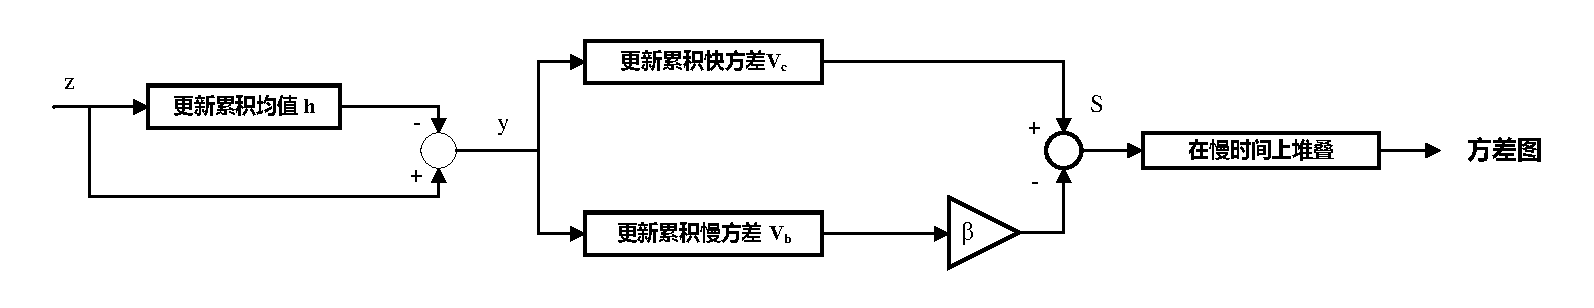
\includegraphics[width=.95\linewidth]{imported/方差图生成流程}
    \caption{\label{fig:variance_graph_pipline}方差图生成流程}
\end{figure}
当场景中出现移动对象时,它会在累积的CIR中产生具有较高方差的区域。通过分析方差图,深度学习算法可以检测到由对象的移动产生的特定模式。图\ref{fig:variance_graph_pipline}中说明了方差图生成的流程,其各个步骤如下所述。

\subsubsection{均值滤波}
由于数据已经过上采样和插值,因此均值滤波比以前\cite{Ledergerber}的方法更简单,但效果更好。我们使用累积均值来计算均值,如下所示:
\begin{equation}
    h = 0.95h + 0.05z
\end{equation}
其中,系数 \( h \) 用第一个接收到的测量值 \( z \) 初始化为 \( h = z \)。

\subsubsection{累积方差}
有了均值以后,可以进一步得到当前测量的CIR的方差度量。这一步也比以前\cite{Ledergerber}的方法更简单。我们使用两个累积均值来跟踪当前和背景方差:
\begin{align}
    V_c &= 0.9V_c + 0.1y \\
    V_b &= 0.999V_b + 0.001y
\end{align}

\subsubsection{背景减除}
通过从当前方差度量中减去背景方差度量,可以检测到CIR中具有暂时较高方差的区域,公式如下:
\begin{equation}
    S = V_c - 1.3V_b
\end{equation}
完成这三个步骤后,生成了每个样本的方差,最后本文在慢时间对样本进行堆叠,生成方差图。


\chapter{定位}

\chapter{脚踢}

\section{引言}
\section{采集设备}
(to do: 
缺少实物图:板子的样子,装在盒子里也可以,如果可以的话可以拍一个装在盒子里的和没在盒子里的
安装图片:可以的话摆拍一下,放在保险杠下面就好,不用太放进去
功能介绍: 就很简短的关于数字钥匙的功能,如果有什么宣传手册给我来一份就好,我可以自己整理

)
\section{数据采集与预处理}
\subsection{CAN数据转化}
控制器局域网络(Controller Area Network, CAN)是一种被广泛应用于汽车、工业自动化和航空电子等领域的网络通讯协议。
CAN总线技术自1980年代由博世(Bosch)公司开发以来,已经成为实现设备之间高效、可靠通信的重要技术。
它通过提供一种低成本、高效且可靠的通信解决方案,极大地推动了现代汽车和工业自动化系统的发展。CAN总线是车辆总线领域的国际标准(ISO 11898)\cite{Chen2009ResearchOT}。

CAN总线技术具有以下几个特点:首先,其具有高效的通信能力,能够在噪音环境中保持稳定的通信。
其次,CAN总线提供了一种简单而灵活的网络架构,可以轻松地将新设备添加到现有的网络中。
再者,通过使用错误检测和错误处理机制,CAN总线能够确保通信的可靠性和实时性。
最后,由于其开放的标准和广泛的支持,CAN总线技术得以在众多不同领域得到应用。

本文使用的超宽带数字钥匙就是通过CAN总线与车辆的电子控制单元(Electronic Control Unit, ECU)进行通讯的,
在开发过程中,本文使用电脑运行python程序,采集通过USB CAN转换器接收到的CAN数据,CAN数据里封装了脚踢检测所需要的CIR信息。

USB CAN转换器实现了CAN总线与USB总线的转换,该设备提供python库文件,可以通过已有的API函数实现CAN数据的接收和发送。
在开发阶段,本文使用电脑通过USB CAN转换器来读取CAN数据,以及运行脚踢检测的算法。开发完成以后,只需要使用嵌入式Linux设备的CAN API函数代替USB CAN设备的函数即可完成迁移。
通过该设备接收到的数据格式如下所示:

\noindent
\begin{minipage}{.5\textwidth}
    \begin{table}[H]
        \caption{\label{tab:Header}消息头格式}
        \centering
        \begin{tabular}{|l|l|}
        \hline
        Field Name & Size \\
        \hline
        Magic Number & 2 bytes \\
        \hline
        Data Count & 4 bytes \\
        \hline
        Paddings & 2 bytes \\
        \hline
        \end{tabular}
    \end{table}
\end{minipage}%
\begin{minipage}{.5\textwidth}
    \begin{table}[H]
        \caption{\label{tab:Payload}消息体格式}
        \centering
        \begin{tabular}{|l|l|}
        \hline
        Field Name & Size \\
        \hline
        Index Number & 1 byte \\
        \hline
        Payload & 7 bytes \\
        \hline
        \end{tabular}
    \end{table}
\end{minipage}
\vspace{\baselineskip} % Adds one line of vertical space

其中,消息头部分的Magic Number为85 85,Data Count记录了采集到的CIR的长度,Paddings是2个字节的无效数据。消息体部分Index Number记录了这是某个消息头下的第几个CAN包,Payload部分记录了真正的CIR数据。
每次采集到的CIR数据的长度是31个复数,每个复数由实部和虚部组成,实部占2个字节,虚部占两个字节。本文通过python程序把CAN数据包转换成其代表CIR的复数数组。

\subsection{训练集采集}
\begin{figure}[htbp]
    \centering
    \begin{subfigure}{0.45\textwidth}
        \centering
        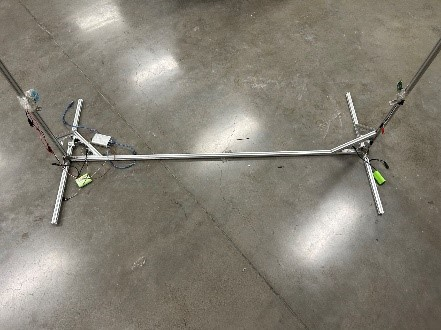
\includegraphics[width=1.0\textwidth]{imported/lab}
        \caption{\label{fig:lab}实验室布置}
    \end{subfigure}%
    \centering
    \begin{subfigure}{0.45\textwidth}
        \centering
        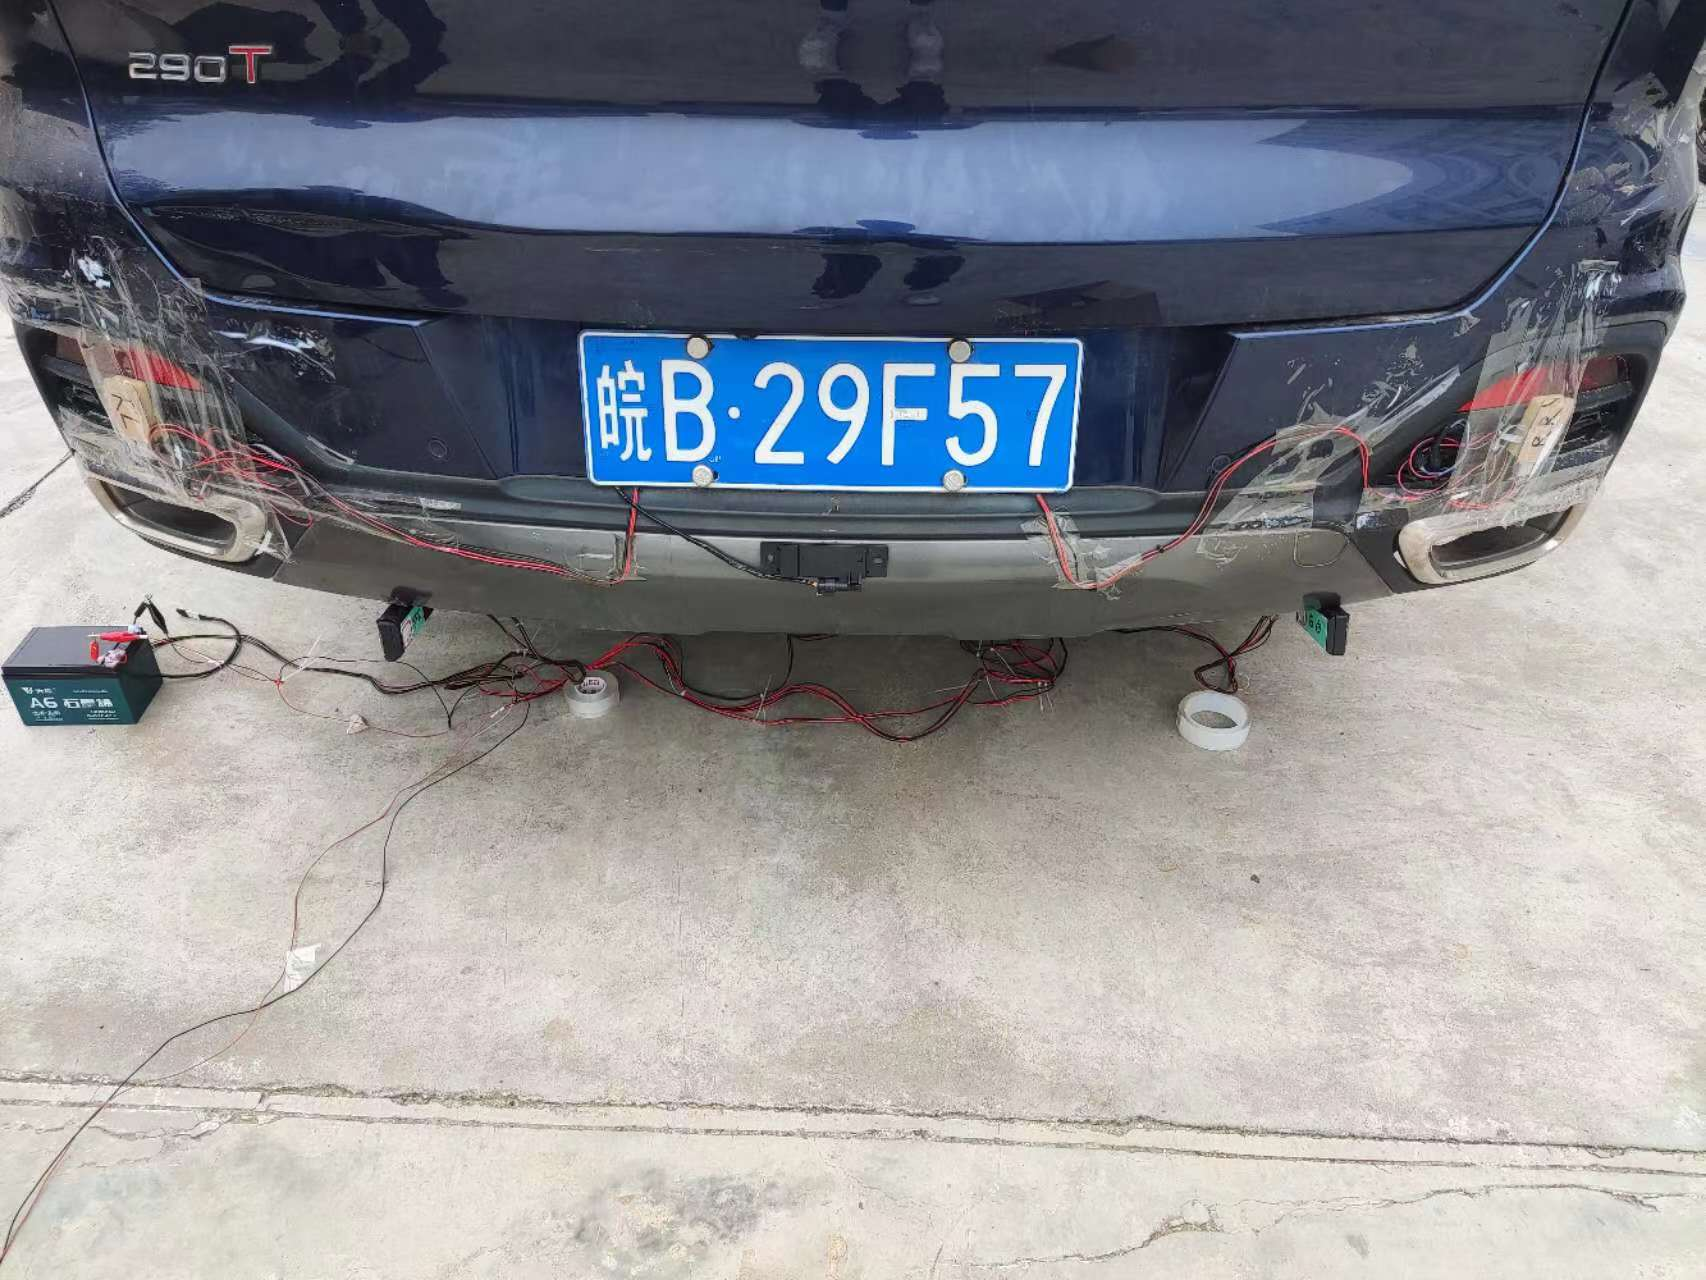
\includegraphics[width=1.0\textwidth]{imported/car}
        \caption{\label{fig:car}实车布置}
    \end{subfigure}%
    \caption{采集设备布置图}
    \label{fig:lab_car_setup}
\end{figure}
如图\ref{fig:lab_car_setup}所示,我们分别在实验室和实车上进行了实验,实验使用了两个NXP NCJ\-29D5设备,其中一个作为发送器,另一个作为接收器。
NXP NCJ29D5的频率范围为6.0 GHz至8.5 GHz。
我们的计算机持续从USB CAN中接收CAN报文并转化成CIR数据。
NXP NCJ29D5每秒生成20个CIR样本。
在训练和测试中,数据经过上述所有处理步骤,并存储为对应于6通道图片的3维数组。

为了训练我们的模型,我们从七个个体收集了数据,每个人进行大约150次水平扫腿。
每次扫腿大约持续2秒,我们通过点击鼠标记录了扫腿开始的时间,以及扫腿结束的时间,从而标注出正样本的位置。
我们手工挑选了特征强烈且清晰的数据。我们选择水平扫腿,因为它们最大化了UWB信号通道上的干扰,从而产生更清晰的信号。
为了减少误报,我们在空白背景环境中,以及人们站立、走路、跑步、跺脚或跳跃时收集负样本。我们总共收集了693个负样本。

为了验证,我们收集了120个水平扫腿样本和120个其他活动的样本,每个样本有20个。我们选择了一个没有参与训练数据收集的人来记录验证数据。

在实验室中,我们使用一个铝支架将设备固定在1.6米的距离上,离地0.3米,以模拟汽车部署。我们将测试系统放在一个相对开放的区域,并使用两个12V电池供电。图7显示了实验室的设置。
在真实的汽车部署中,我们将设备放置在汽车的后备箱下方一米处,天线面向汽车的后部,以最大化信号质量并最小化对其原始数字钥匙功能的干扰。
在这两种情况下,传感器和被检测对象之间的距离均在0.4米以内。

\subsection{数据集生成}
  
\section{模型设计}
\section{模型训练}
(to do: 在此处放置tensorboard产生的loss,metrics随着训练进行变化的图片)

\section{模型部署}





\chapter{呼吸}

\chapter{总结与展望}

\chapter{关于本模板}

本模板根据浙江大学研究生院编写的《浙江大学研究生学位论文编写规则》~\cite{zjugradthesisrules},
在原有的 zjuthesis 模板~\cite{zjuthesis}基础上开发而来。

本模板的本科生版本\cite{zjuthesisrules}得到了浙江大学本科生院老师的支持与审核,
已经在本科生院网上公示。
但当前的研究生版本并未经过研究生院老师的审核,
同学们使用时要注意对照模板与要求,
切不可盲目使用。

作者本人并未编写过浙江大学研究生毕业论文,
所以不清楚具体要求。
如果有热心同学愿意帮忙,
可以替我联系相关老师,我会配合审核并修改代码。

\section{Overleaf 使用注意事项}

如果你在Overleaf上编译本模板,请注意如下事项:

\begin{itemize}
    \item 删除根目录的 ``.latexmkrc'' 文件,否则编译失败且不报任何错误
    \item 字体有版权所以本模板不能附带字体,请务必手动上传字体文件,并在各个专业模板下手动指定字体。
          具体方法参照 GitHub 主页的说明。
    \item 当前的Overleaf默认使用TexLive 2017进行编译,但一些伪粗体复制乱码的问题需要TexLive 2019版本来解决。
          所以各位同学可以在Overleaf上编写论文时务必切换到TexLive 2019或更新版本来编译,以免产生查重相关问题。
          具体说明参照 GitHub 主页。
\end{itemize}


\section{节标题}

我们可以用includegraphics来插入现有的jpg等格式的图片,
如\autoref{fig:zju-logo}所示。

\begin{figure}[htbp]
    \centering
    \includegraphics[width=.3\linewidth]{logo/zju}
    \caption{\label{fig:zju-logo}浙江大学LOGO}
\end{figure}


\subsection{小节标题}


\par 如\autoref{tab:sample}所示,这是一张自动调节列宽的表格。

\begin{table}[htbp]
    \caption{\label{tab:sample}自动调节列宽的表格}
    \begin{tabularx}{\linewidth}{c|X<{\centering}}
        \hline
        第一列 & 第二列 \\ \hline
        xxx & xxx \\ \hline
        xxx & xxx \\ \hline
        xxx & xxx \\ \hline
    \end{tabularx}
\end{table}


\par 如\autoref{equ:sample},这是一个公式

\begin{equation}
    \label{equ:sample}
    A=\overbrace{(a+b+c)+\underbrace{i(d+e+f)}_{\text{虚数}}}^{\text{复数}}
\end{equation}

\chapter{另一章}


\begin{figure}[htbp]
    \centering
    \includegraphics[width=.3\linewidth]{example-image-a}
    \caption{\label{fig:fig-placeholder}图片占位符}
\end{figure}

\chapter{再一章}

\par 如\autoref{alg:sample},这是一个算法

\begin{algorithm}[H]
    \begin{algorithmic} % enter the algorithmic environment
        \REQUIRE $n \geq 0 \vee x \neq 0$
        \ENSURE $y = x^n$
        \STATE $y \Leftarrow 1$
        \IF{$n < 0$}
        \STATE $X \Leftarrow 1 / x$
        \STATE $N \Leftarrow -n$
        \ELSE
        \STATE $X \Leftarrow x$
        \STATE $N \Leftarrow n$
        \ENDIF
        \WHILE{$N \neq 0$}
        \IF{$N$ is even}
        \STATE $X \Leftarrow X \times X$
        \STATE $N \Leftarrow N / 2$
        \ELSE[$N$ is odd]
        \STATE $y \Leftarrow y \times X$
        \STATE $N \Leftarrow N - 1$
        \ENDIF
        \ENDWHILE
    \end{algorithmic}
    \caption{\label{alg:sample}算法样例}
\end{algorithm}